\documentclass{beamer} 
\usepackage{amsmath,amsthm}
\usepackage{graphicx,microtype,parskip}
\usepackage{caption,subcaption,multirow}
\usepackage{attrib}

\frenchspacing

\usetheme{default}
\usecolortheme{whale}

\setbeamertemplate{navigation symbols}{}

\setbeamercolor{title}{fg=blue,bg=white}

\setbeamercolor{block title}{fg=white,bg=gray}
\setbeamercolor{block body}{fg=black,bg=lightgray}

\setbeamercolor{block title alerted}{fg=white,bg=darkgray}
\setbeamercolor{block body alerted}{fg=black,bg=lightgray}

%\AtBeginSection[]
%{
%  \begin{frame}
%    \tableofcontents[currentsection]
%  \end{frame}
%}

\title{How macroecology affects macroevolution}
\subtitle{the interplay between extinction intensity and trait-dependent extinction in brachiopods}
\author{Peter D Smits}
\institute{Committee on Evolutionary Biology, University of Chicago}
\titlegraphic{
  
\includegraphics[width=2.75cm,height=2.75cm,keepaspectratio=true]{figure/paleodb}
  \hspace*{0.35\paperwidth}
  
\includegraphics[width=2cm,height=2cm,keepaspectratio=true]{figure/chicago}
}
\date{}

\begin{document}

\begin{frame}
  \maketitle
\end{frame}

\begin{frame}
  \begin{alertblock}{Observation}
    At K/Pg mass extinction, biological traits (except geographic range) have no effect on \alert{bivalve} taxonomic survival.

    \attrib{\footnotesize{Jablonski, 1986, \em{Science}}}
  \end{alertblock}
\end{frame}



\begin{frame}
  \frametitle{Intensity and selectivity}

\end{frame}



\begin{frame}
  \begin{alertblock}{Questions and analysis}
    \begin{itemize}
      \item How do the effect of emergent traits on duration (\alert{extinction selectivity}) vary with expected duration (\alert{extinction intensity}) and each other?
      \item What is the relationship between environmental affinity and duration wrt specialists versus generalists?
      \item \textbf{Approach:} hierarchical Bayesian survival model, \\varying intercepts and slopes, Weibull distribution, \\imputed gap statistic for taxa with duration \(< 3\).
    \end{itemize}
  \end{alertblock}
\end{frame}



\begin{frame}
  \frametitle{Analysis of post-Cambrian Paleozoic brachiopod genus durations}
  \begin{itemize}
    \item stage as time unit; duration measured in stages
    \item multiple emergent traits analyzed
      \begin{itemize}
        \item geographic range
          \begin{itemize}
            \item transformed using \textbf{JADE} fo biased sampling \\(Chao et al. 2015 \textit{Ecology})
          \end{itemize}
        \item body size
          \begin{itemize}
            \item from Payne et al from the \textit{Treatise on Invertebrate Paleontology}
          \end{itemize}
        \item environmental preference (x, x\(^2\))
        \item gap statistic as measure of sampling (Foote and Raup 1996 \textit{Paleobio})
      \end{itemize}
    \item factors vary by cohort (except gap statistic)
  \end{itemize}
\end{frame}


\begin{frame}
  \frametitle{Relationship between range size and extinction risk}

  % abstract diagram

\end{frame}


\begin{frame}
  \frametitle{Hypotheses of effect of environmental preference}
  \begin{quote}
    When related phyla die out \dots more specialized phyla tend to become extinct before less specialized. This phenomenon is also far from universal, but it is so common that it does deserve recognition as a rule or principle in evolutionary studies: \textbf{the rule of the survival of the relatively unspecialized.}

    \attrib{\footnotesize{Simpson, 1944, \em{Tempo and Mode of Evolution}, p. 143}}
  \end{quote}
\end{frame}

\begin{frame}
  \begin{block}{New measure of taxon's environmental affinity}
    (\# epicontinental / total \# occurrences) is what quantile of the distribution of all other background occurrences Beta(\(\alpha\), \(\beta\)).
    \begin{itemize}
      \item \(\alpha\) is the \# epicontinental background occurrences (+ 1).
      \item \(\beta\) is the \# open ocean background (+ 1).
    \end{itemize}
  \end{block}
\end{frame}

\begin{frame}
  \frametitle{Hypotheses of effect of environmental breadth}
  \begin{center}
    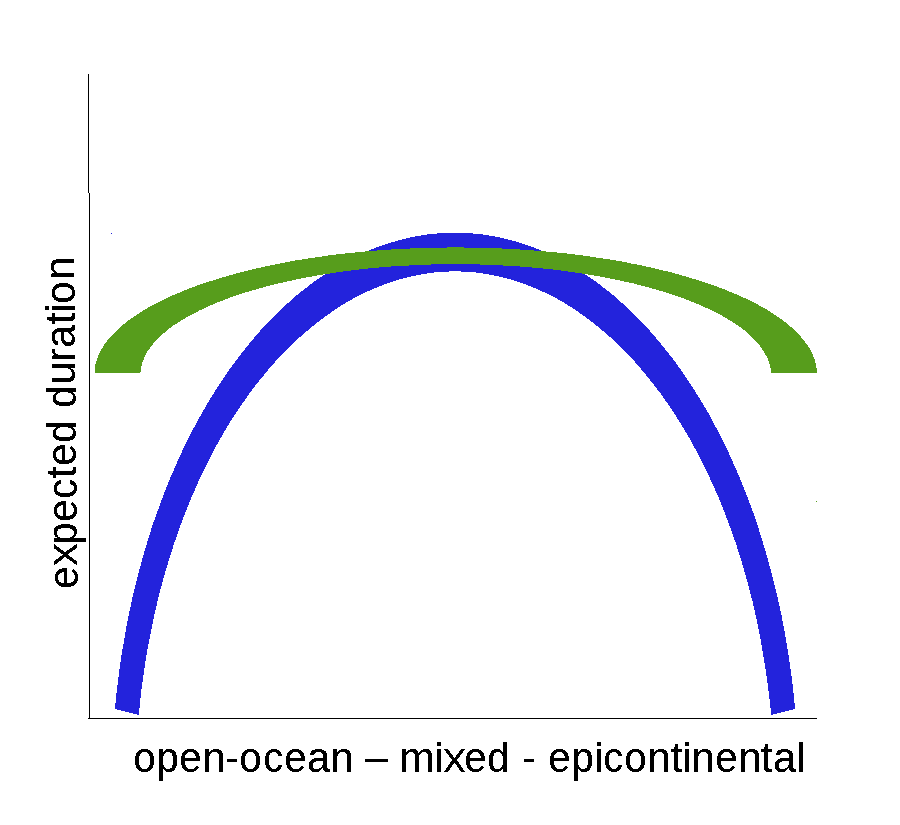
\includegraphics[width = \textwidth,height = 0.8\textheight,keepaspectratio = true]{figure/selection_breadth}
  \end{center}
\end{frame}


\begin{frame}
  \begin{block}{Measure of sampling and imputed values}
    Sampling is measured as the gap statistic \(r\): \\(number of bins with an occurrence - 2) / (duration in bins - 2)

    Can only be estimated for taxa with duration of three or more. \\Have to impute (e.g. fill-in) the values for all other taxa \(r^{\ast}\).
    \begin{align*}
      s &\sim \text{Beta}(\phi, \lambda) \\
      \phi &= \text{logit}^{-1}(W\gamma) \\
      s^{\ast} &\sim \text{Beta}(\phi^{\ast}, \lambda) \\
      \phi^{\ast} &= \text{logit}^{-1}(W^{\ast}\gamma) \\
    \end{align*}
    \scriptsize{Note: Beta distribution parameterized in terms of mean \(\phi\) and total count \(\lambda\). \\Also, this presentation excludes final (hyper)priors.}
  \end{block}
\end{frame}


\begin{frame}
  \frametitle{Hierarchical survival model}
  \begin{center}
    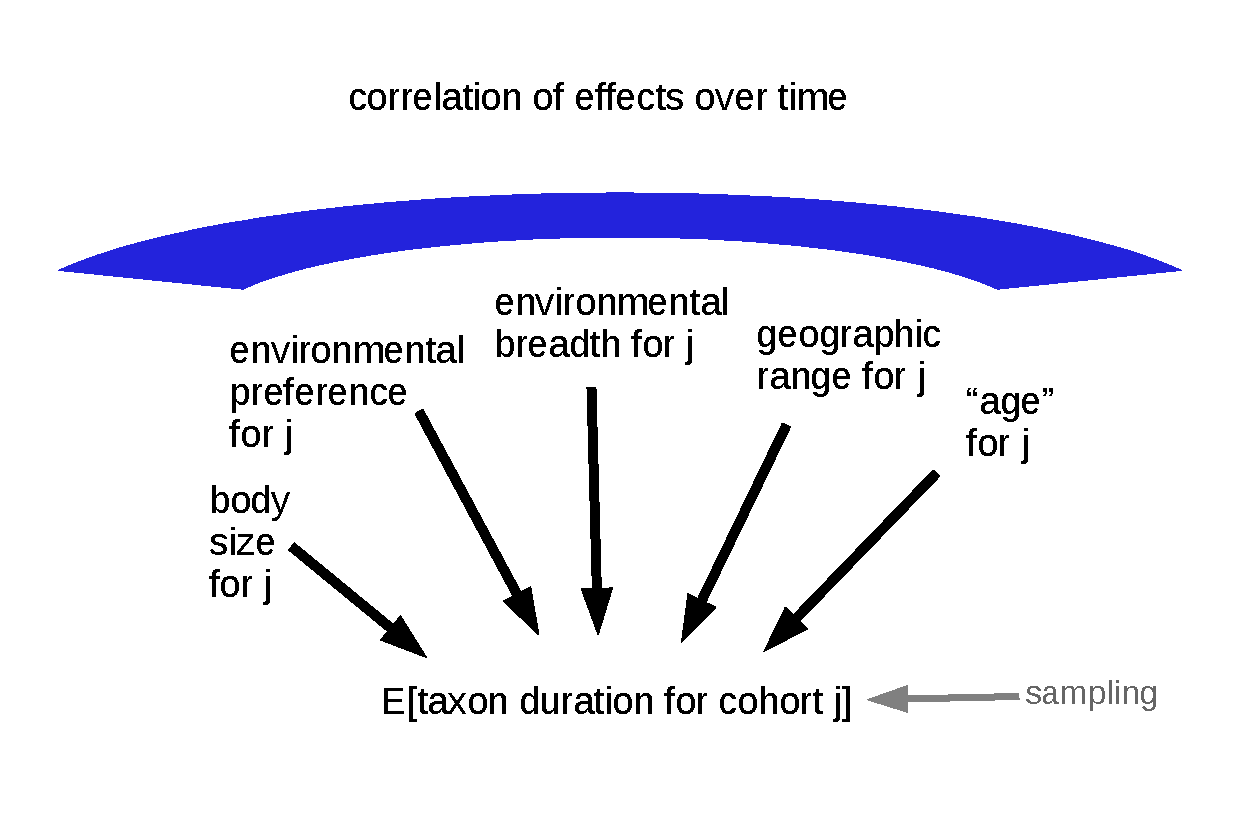
\includegraphics[width = \textwidth,height = 0.8\textheight,keepaspectratio = true]{figure/simple_model}
  \end{center}
\end{frame}


\begin{frame}
  \frametitle{Model adequacy}
  \begin{columns}
    \begin{column}{0.5\textwidth}
      \begin{center}
        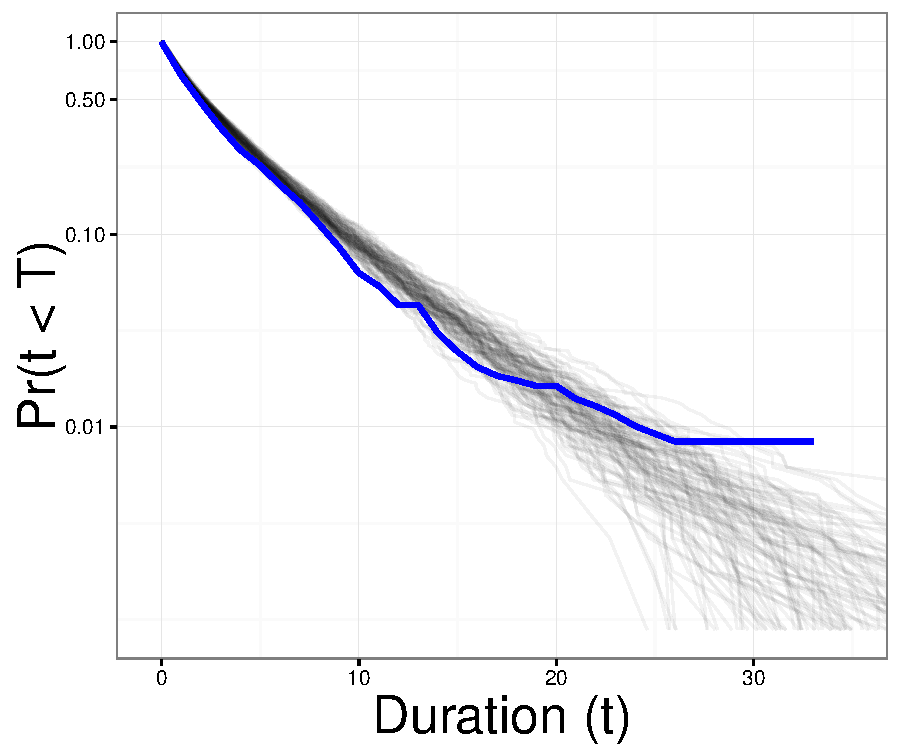
\includegraphics[width=\textwidth,height=0.8\textheight,keepaspectratio=true]{figure/survival_curves}
      \end{center}
    \end{column}
    \begin{column}{0.5\textwidth}
      \begin{center}
        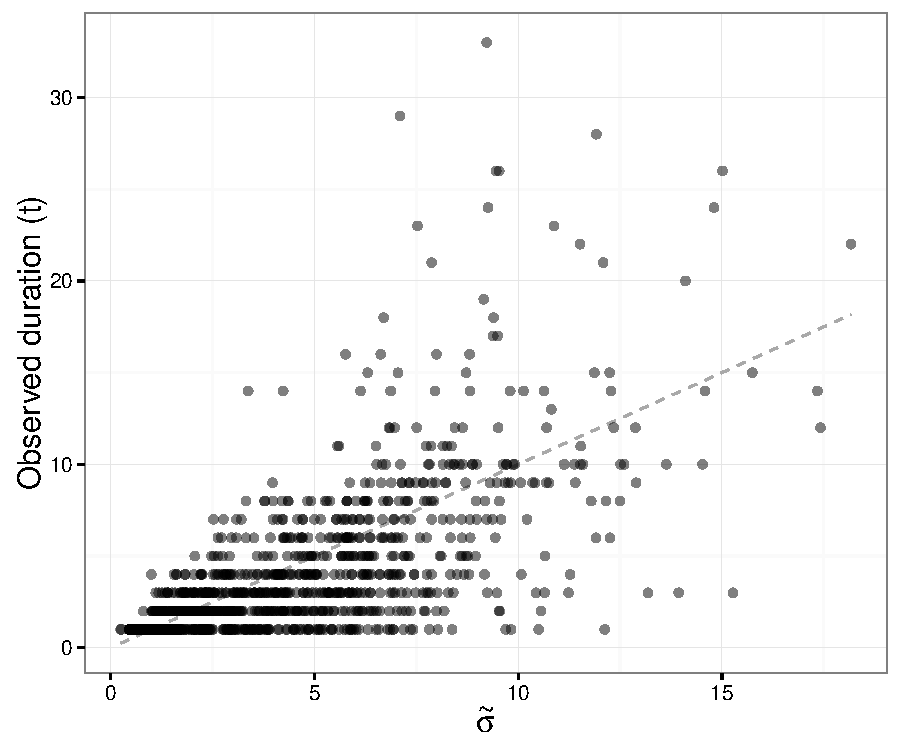
\includegraphics[width=\textwidth,height=0.8\textheight,keepaspectratio=true]{figure/shotgun}
      \end{center}
    \end{column}
  \end{columns}
\end{frame}

\begin{frame}
  \frametitle{Inspecting the imputations}
  \begin{center}
    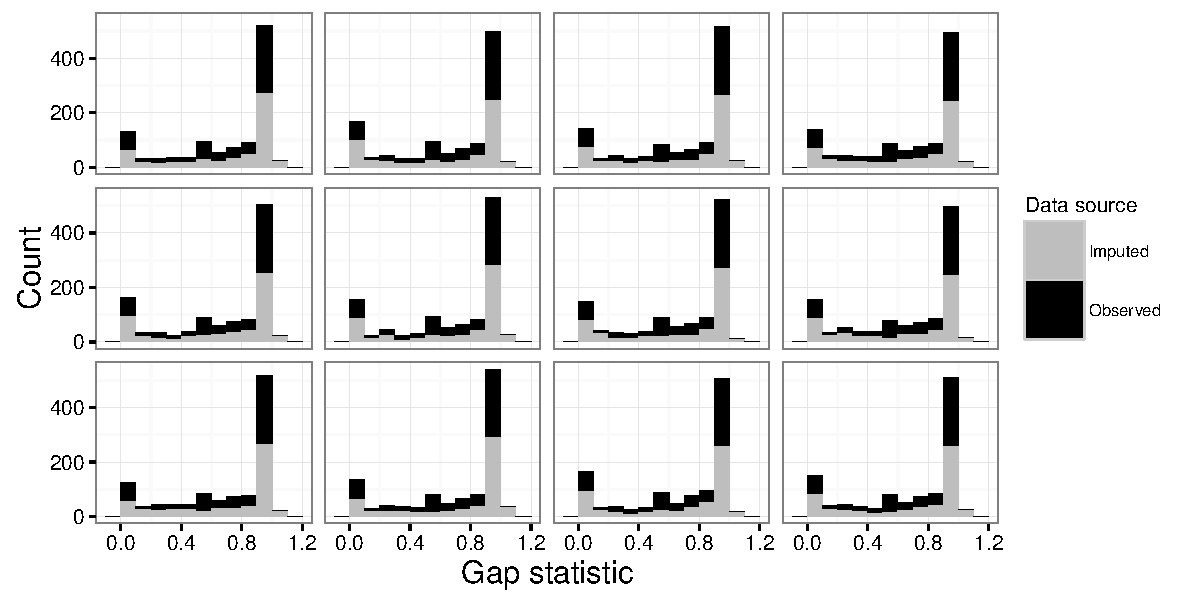
\includegraphics[width=\textwidth,height=0.8\textheight,keepaspectratio=true]{figure/imputation_compare}
  \end{center}
\end{frame}


\begin{frame}
  \frametitle{Change in trait effects between cohorts}

  \begin{center}
    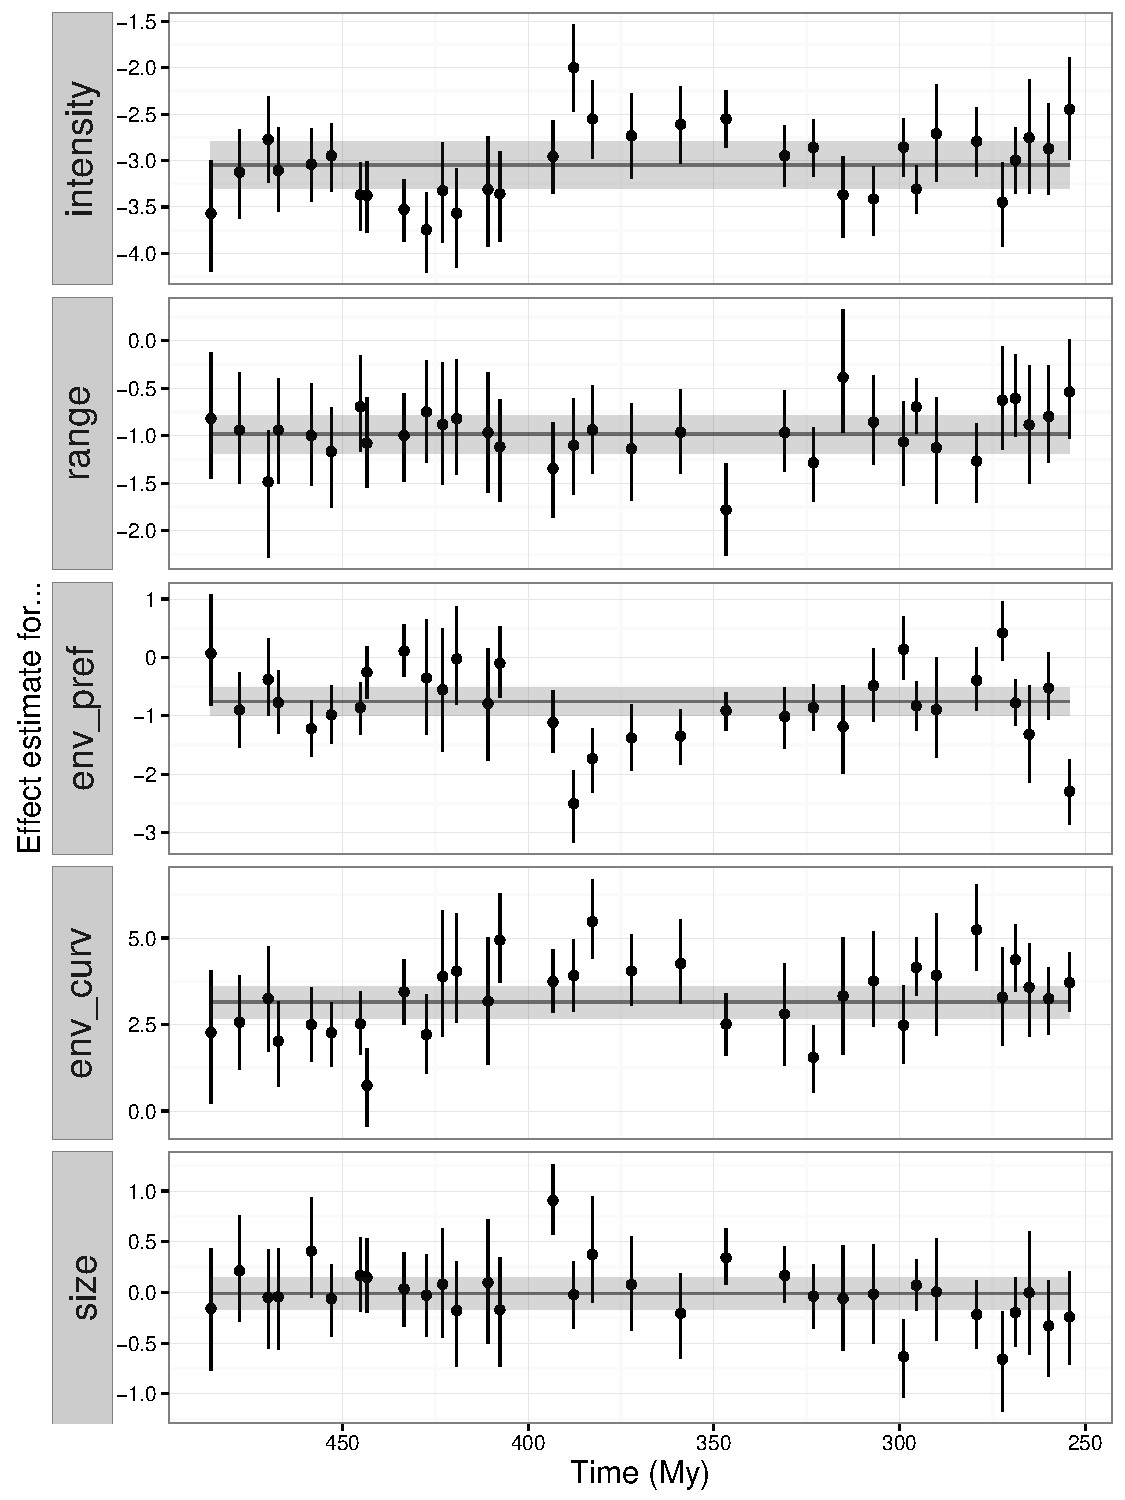
\includegraphics[width = \textwidth,height = 0.8\textheight,keepaspectratio = true]{figure/cohort_series}
  \end{center}
\end{frame}

\begin{frame}
  \frametitle{Overall effect of environmental preference}

  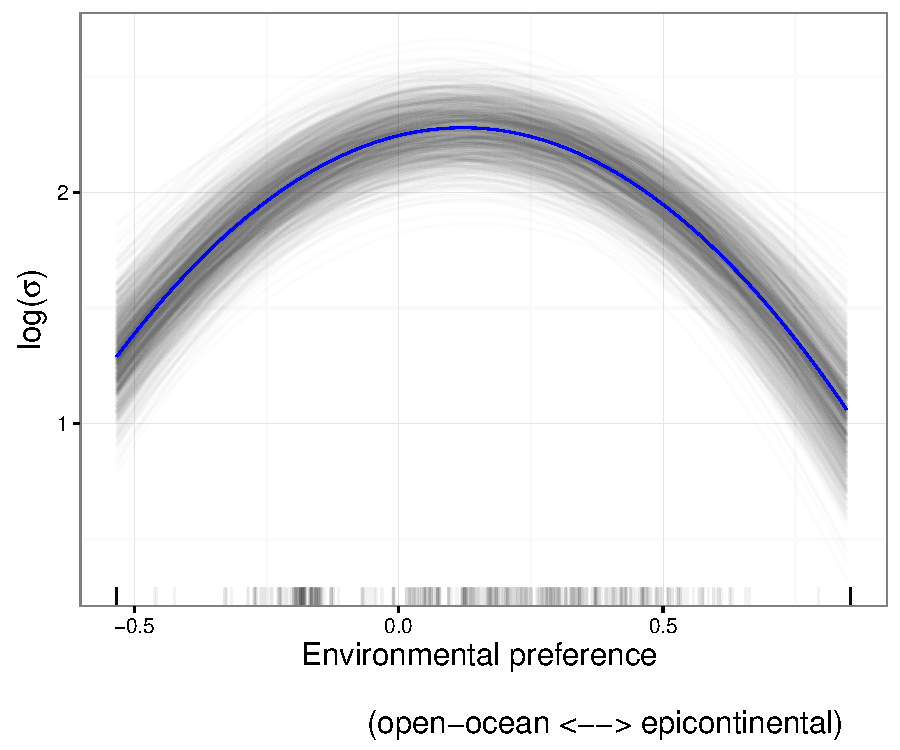
\includegraphics[width = \textwidth,height = 0.8\textheight,keepaspectratio = true]{figure/env_effect}
\end{frame}

%\begin{frame}
%  \frametitle{Change in effect of environment between cohorts}
%
%  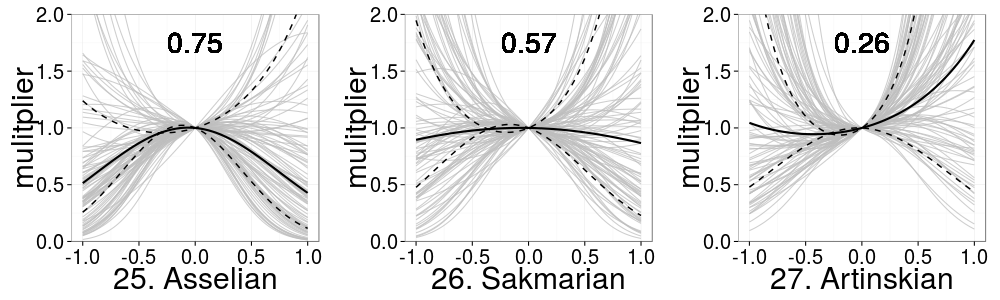
\includegraphics[width = \textwidth,height = \textheight,keepaspectratio = true]{figure/cohort_quads_short}
%\end{frame}

\begin{frame}
  \frametitle{Change in effect of environment between cohorts}

  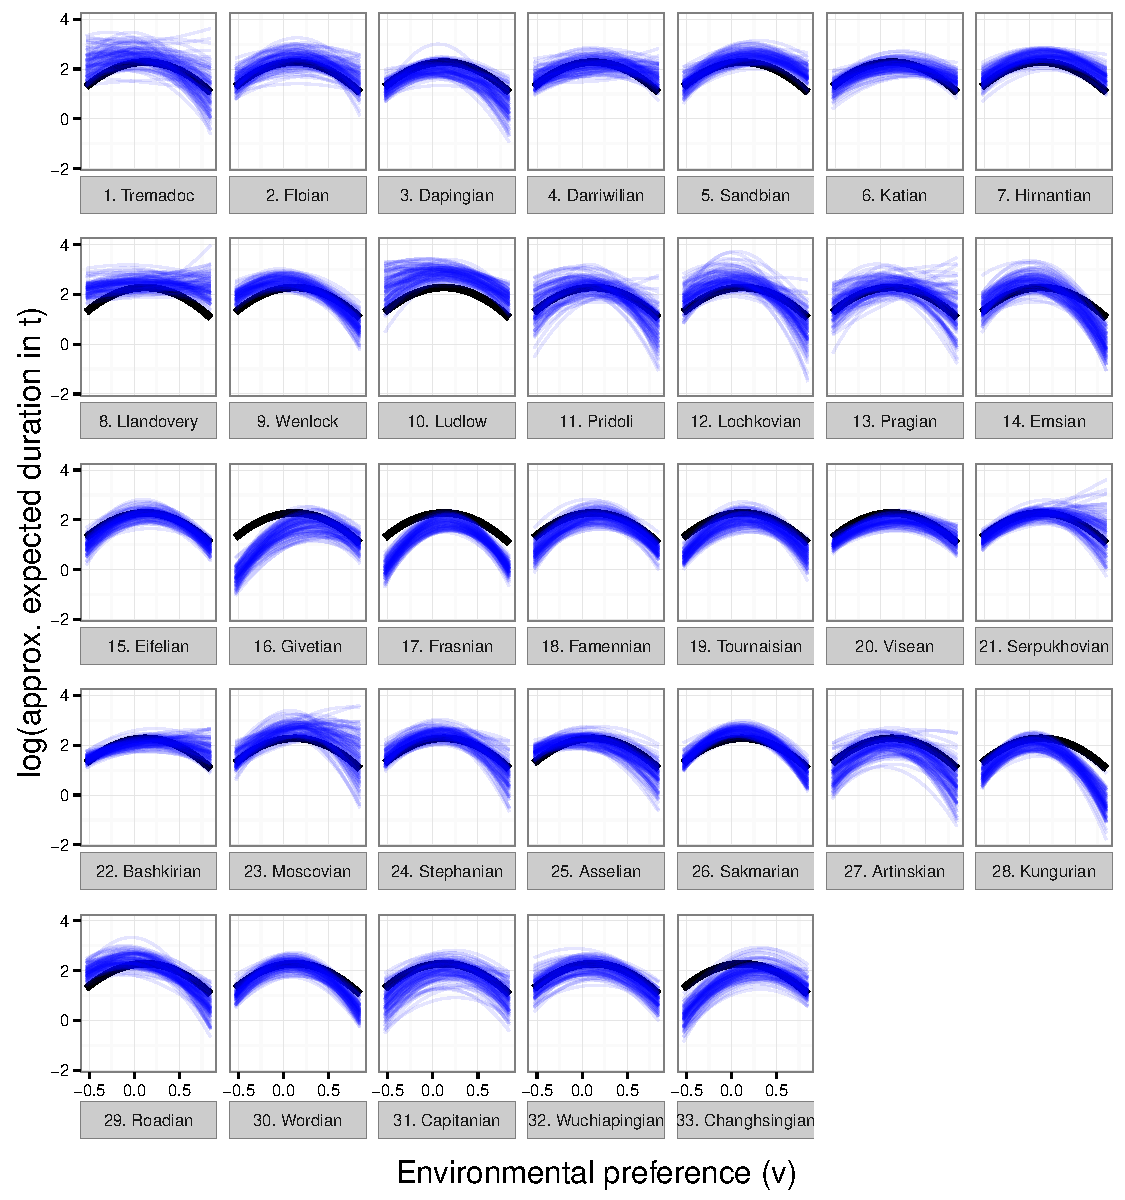
\includegraphics[width = \textwidth,height = \textheight,keepaspectratio = true]{figure/env_cohort}
\end{frame}

\begin{frame}
  \frametitle{Correlation of effects between cohorts}

  \begin{center}
    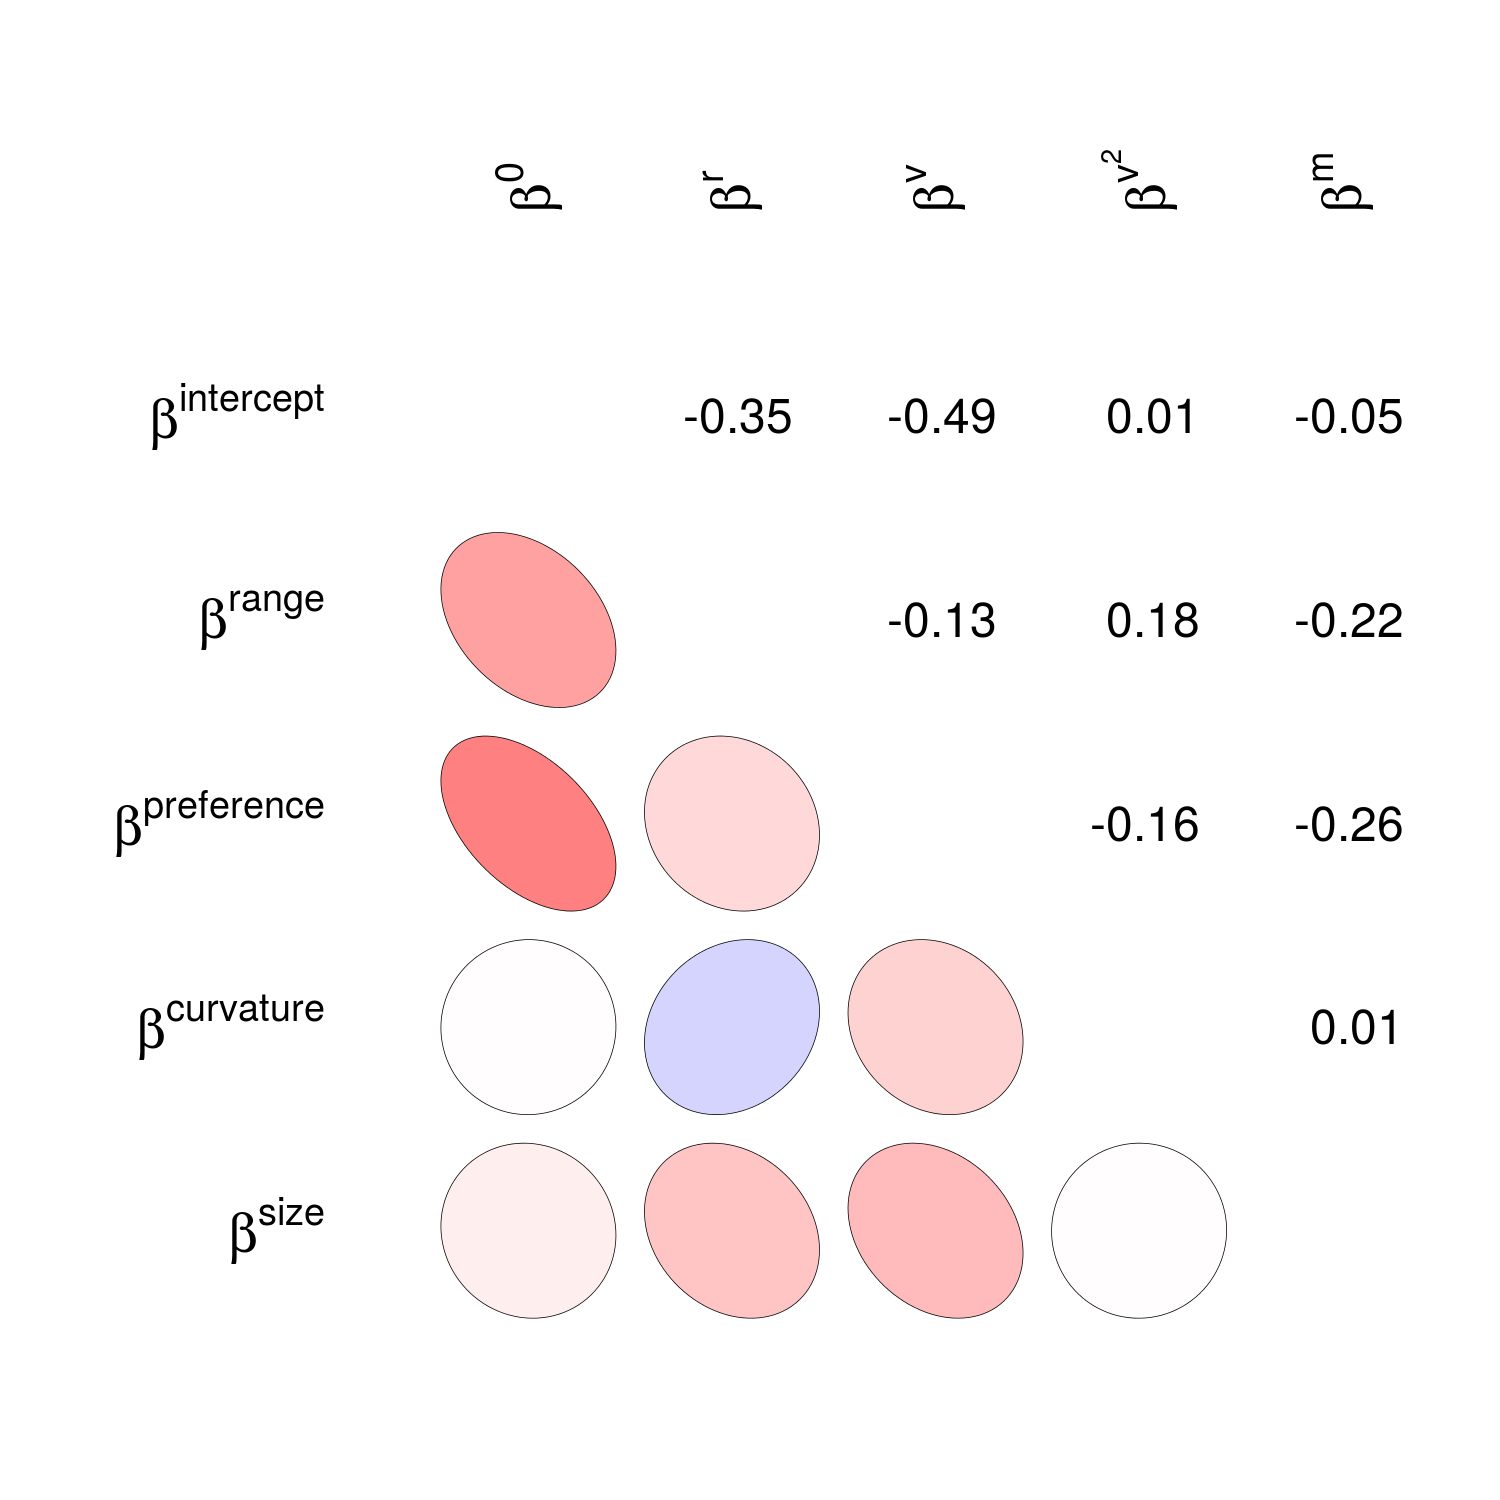
\includegraphics[width = \textwidth,height = 0.9\textheight,keepaspectratio = true]{figure/wei_cor_heatmap}
  \end{center}
\end{frame}

\begin{frame}
  \begin{block}{Effect summary}
    \begin{itemize}
      \item Effect of geographic range consistent with prior expectations.
      \item No effect of body size; environmental preference equal.
      \item Weak support for survival of unspecialized as generalization.
    \end{itemize}
  \end{block}
\end{frame}

\begin{frame}
  \begin{block}{Correlation of effects}
    \begin{itemize}
      \item Correlation between baseline extinction risk and effects of geographic range as well as environmental breadth.
      \item Correlation between effect of range and effect of environmental breadth.
        \begin{itemize}
          \item As effect of geographic range increases, decrease in selection on environmental breadth.
        \end{itemize}
    \end{itemize}
  \end{block}
\end{frame}

\begin{frame}
  \begin{alertblock}{Macroevolutionary process}
    \begin{itemize}
      \item As extinction risk increases, the effect of geographic range ``washes out'' the effects of other traits.
        \begin{itemize}
          \item Support for hypotheses presented in Jablonski 1986 Science, Raup 1994 PNAS.
        \end{itemize}
    \end{itemize}
  \end{alertblock}
\end{frame}

\begin{frame}
  \frametitle{Acknowledgements}
  \begin{columns}
    \begin{column}{0.5\textwidth}
      \begin{itemize}
        \item Advising
          \begin{itemize}
            \item Kenneth D. Angielczyk, Michael J. Foote, \\P. David Polly, \\Richard H. Ree, \\Graham Slater
          \end{itemize}
        \item Angielczyk Lab
          \begin{itemize}
            \item {\small{David Grossnickle, \\Dallas Krentzel, \\Jackie Lungmus}}
          \end{itemize}
        \item Foote lab
          \begin{itemize}
            \item {\small{Marites Villarosa Garcia, \\Nadia Pierrehumbert}}
          \end{itemize}
      \end{itemize}
    \end{column}
    \begin{column}{0.5\textwidth}
      \begin{itemize}
        \item {\footnotesize{Stewart Edie, \\Elizabeth Sander, \\Laura Southcott, \\Courtney Stepien}}
        \item {\footnotesize{David Bapst, \\Ben Frable, \\\textbf{Arnold Miller}, \\Peter Wagner}}
      \end{itemize}

      \vspace*{0.05\textheight}
      \begin{center}
        
\includegraphics[height=0.2\textheight,width=\textwidth,keepaspectratio=true]{figure/paleodb}
      \end{center}
    \end{column}
  \end{columns}
\end{frame}

\end{document}
